\section{编码风格}
国际上有一项有趣的比赛,名为国际C语言混乱代码大赛(International Obfuscated C Code Contest, IOCCC)。此项比赛的宗旨在于鼓励人们写出最有创意和最让人难以理解的C语言代码。图7.3就是一个这样的例子(代码部分),它的代码是一个飞行器的形状,而运行结果也是一个飞行模拟器。\par
\begin{figure}[htbp]
    \centering
    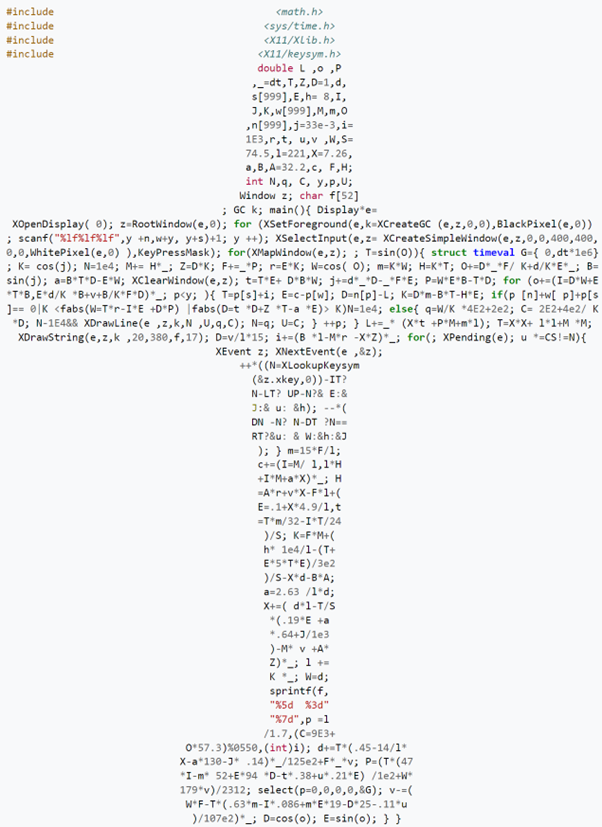
\includegraphics[width=.8\textwidth]{../images/generalized_parts/07_international_obfuscated_c_code_contest_instance.png}
    \caption{飞行模拟器(1998年IOCCC获奖作品)的代码}
    \footnotesize{资料来源:Wikipedia}
\end{figure}
这份代码很复杂,而且很难懂,非常合乎``有创意''和``难以理解''的宗旨。而这也正是我们在日常写代码时要规避的,否则无论是写代码时检查逻辑,还是写完代码复盘内容,抑或是交给别人学习,这样难懂的代码都会给人增加诸多不必要的麻烦。\par
它难以理解的方面主要有以下几点:
\begin{itemize}
    \item 排版混乱。虽然这个排版很有创意,但这也使得我们在阅读时难以理清代码之间的逻辑。
    \item 命名混乱。这段代码用了各种简短的名字,比如 \lstinline@L@, \lstinline@o@ 甚至 \lstinline@_@ 这样的名字!命名不清很容易导致人在阅读代码时不知所云。
    \item 语句臃肿。在很多地方,硬生生地把一个复杂功能用单一的语句表达出来,这样就会让代码变得十分难懂。
    \item 完全没有注释。很多人十分反感在代码中写注释,觉得很麻烦——我自己就是如此。但是有效的注释可以大大增加代码的可读性。很多时候,我们用一句话就可以表达清楚一个函数的作用,比把代码写得清楚还要有用。
\end{itemize}
那么我们就根据这个``反面教材'',来讲一下如何写一段令人赏心悦目的代码。\par
\subsubsection*{代码排版}
在排版方面,适当的空格、缩进和换行能让代码更易读。空格的作用很明显,它可以将逻辑上不同的事物区分开来(很多时候,仅靠运算符来进行区分还不够清晰)。以下是一个对比:
\begin{lstlisting}
//无空格
    for(i=0;i<10;++i)
        std::cout<<arr[i].member;
//有空格
    for (i = 0; i < 10; ++i)
        std::cout << arr[i].member;
\end{lstlisting}
注意这里的 \lstinline@std::cout@ 和 \lstinline@arr[i].member@ 之间没有空格,其实也可以有。我的理解是:这里不需要空格,因为它们是用来表示同一个事物的,所以不需要用空格来区分开。读者当然也可以有自己的理解,并逐渐形成自己的风格,只要它易读就好了。\par
对于缩进和换行来说,不同代码风格的习惯更是迵异——不过大体原则还是相似的,无非是在花括号是否换行、标签是否不缩进等细节上有出入。\par
斯特劳斯特鲁普在自己的文章\footnote{\href{https://www.stroustrup.com/Programming/PPP-style.pdf}{\textit{PPP Style Guide} - Bjrane Stroustrup}}中简单介绍了一种C++编码风格,它是对K\&R风格\footnote{K\&R风格(Kernighan \& Ritchie Style, K\&R style)是一种常见于C/C++等花括号编程语言的风格,其核心特点在于:首尾花括号与引出花括号的语句保持相同缩进,而花括号内的语句增加一层缩进。}的变体。本书也推荐读者学习和使用这种``斯特劳斯特鲁普变体''\footnote{至于其它的常见编码风格,\href{https://en.wikipedia.org/wiki/Indentation_style\#Brace_placement_in_compound_statements}{Brace placement in compound statements - Wikipedia} 列表中有所介绍。读者也可以挑选一种合自己心意的来使用。}。接下来对它作简要介绍;如果读者希望了解更多,可以去阅读他的文章。\par
一般我们会对逻辑上有附属关系的语句加一层缩进。例如说 \lstinline@if@ 语句的作用域内,就要加一层缩进。
\begin{lstlisting}
if (a > 0)
    std::cout << "Positive";
else if (a < 0)
    std::cout << "Negative";
else
    std::cout << "Zero";
\end{lstlisting}
其它诸如 \lstinline@for@, \lstinline@while@, \lstinline@switch@ 等结构,以及函数定义、类定义等也是如此。\par
再比如,在初始化数组的时候,假如初始化内容非常冗长,我们也可以换行加适当缩进。
\begin{lstlisting}
struct Data {
    int num;
    Data *next;
};
Data heads[3] {
    {0, nullptr},
    {0, nullptr},
    {0, nullptr}
};
\end{lstlisting}
我们这样定义\footnote{补充:全局变量定义在Data段或BSS段。如果我们没有提供初始化的话,它会存储于BSS段,同时获得默认值。这个默认值对于整型来说是 \lstinline@0@,对于指针来说是 \lstinline@nullptr@,因此我们可以只定义 \lstinline@heads[3]@ 但不提供初始化,效果相同。这里只为讲解而如此。},肯定比下面这种写法要美观吧——
\begin{lstlisting}
Data heads[3]{{0, nullptr}, {0, nullptr}, {0, nullptr}};
\end{lstlisting}\par
这些都是常见的缩进原则\footnote{C/C++都是自由格式语言(Free-form language),自由格式语言对空格的要求不太,对缩进和换行则是几乎没有要求;非自由格式语言,如Python,写起来更简洁,但它对格式要求更严格,比如说缩进直接与逻辑挂钩,所以就不能像IOCCC示例那样乱写。}。至于换行,适当的换行配合缩进,也能让程序更加整洁。
\begin{lstlisting}
//写到同一行
if (ch > 'a' && ch < 'z' || ch > 'A' && ch < 'Z' || ch > '0' && ch < '9') {
    //...
}
//适当换行+缩进
if (ch > 'a' && ch < 'z'
    || ch > 'A' && ch < 'Z'
    || ch > '0' && ch < '9'
){
        //...
}
\end{lstlisting}
孰优孰劣,就不言而喻了吧。\par
\subsubsection*{命名}
在写一些小的函数时,我们常常会用一些简短的变量/函数或类名称,比如说
\begin{lstlisting}
template <typename T>
T max(T a, T b) {
    return a > b ? a : b;
}
\end{lstlisting}
但这种习惯最好不要带到大规模函数中,尤其是那种需要数据处理或交互的场合,很容易让人搞不懂一个变量名意味着什么。\par
函数名和类名尤其应当如此。虽然名字是可以随便起的,但最好还是要做到让人顾名思义。标准库中的 \lstinline@max@ 和 \lstinline@strlen@ 函数,\lstinline@string@ 和 \lstinline@list@ 类等,都有这样顾名思义的优点。\par
至于具体的命名,可以用简称(比如有人会用 \lstinline@siz@ 代替 \lstinline@size@,当然这样也可以避免与 \lstinline@std::size@ 撞名,所以也很受常用 \lstinline@using namespace std@ 人士的喜好)或全名。至于我自己写代码时,一般都使用全名(反正我不用 \lstinline@using namespace std@)。读者可以选择自己喜欢的命名风格。
\subsubsection*{语句的处理}
有些程序员对于``压行''有一种执念,能写在一句(一行)代码中的内容,就尽量写在同一句,而不是把它拆成多句(多行)。为了压行,他们可以使用各种手段,比如把嵌套的选择结构用条件运算符拼湊起来,比如:
\begin{lstlisting}
return exp1 ? exp2 ? opt1 : opt2 : exp2 ? opt3 : opt4; //甚至可以继续缝
\end{lstlisting}\par
这种习惯对于稍大规模的项目来说是不利的,因为稍大规模的项目不可避免地会有很多代码,这时最重要的并不是``行数少'',而是代码逻辑一目了然,容易让人(包括自己)看懂。否则一旦代码写出了问题,自己就要费很大事来从这一句冗长的代码当中抽丝剥茧,这是何苦呢?\par
所以,除非这段代码的逻辑简单到可以写成 \lstinline@max@ 那样,否则我们还是老老实把代码的逻辑写得清楚一点,这样能免去很多麻烦。
\begin{lstlisting}
if (exp1) {
    if (exp2) {
        opt1;
    }
    else {
        opt2;
    }
}
else {
    if (exp2) {
        opt3;
    }
    else [
        opt4;
    ]
}
\end{lstlisting}\par
还有一些时候,我们需要表示一个很长的表达式——比如说一元二次方程的求根公式。
\begin{lstlisting}
#include <utility>
#include <cmath>
using std::sqrt;
//把sqrt引入全局命名空间中,这样我们就不用再写std::sqrt了
using pair = std::pair<double, double>;
//pair是一个类模版,它的对象可以存储两个值,适合本例
//这里使用using之后,我们可以直接用pair来代替std::pair<double,double>
pair quadratic_solve(double a, double b, double c) {
    return pair(
        (-b - sqrt(b * b - 4 * a * c)) / 2 / a,
        (-b + sqrt(b * b - 4 * a * c)) / 2 / a
    ); //这里用到了std::pair的构造函数,我们下一章再讲。
}
\end{lstlisting}
这里我们就不管命名的问题了,因为我们在数学上就是用$a,b,c$的,而且这个函数的功能也没有复杂到需要用多少名字。但仅就表达式的形式来看,它也是非常冗长难看的。\par
对于这种,乃至更冗长的表达式,我们最好是用中间变量的方式来简化我们的表达。我们在数学中是用中间变量$\Delta$来表式根式内的部分,而在编程中我们也可以这样做。
\begin{lstlisting}
pair quadratic_solve(double a, double b, double c) {
    const double Delta {b * b - 4 * a * c}; //常量中间变量Delta
    return pair(
        (-b - sqrt(Delta)) / 2 / a,
        (-b + sqrt(Delta)) / 2 / a
    ); //这样写就显得简洁了一些
}
\end{lstlisting}\par
\subsubsection*{注释}
注释的好处,已经不再需要我多作说明了。本书示例代码中的注释详尽之致,想必读者都能感受得到。对于编译器来说,注释部分的内容会被完全忽略,所以注释主要是为了给人看的。\par
良好的注释对于我们理解代码来说很重要,尤其是过了几天到几个月之后,如果你回看源代码,会感谢你当时写过的注释的。\par
C++中允许我们使用行注释和块注释,我们在前文中的绝大部分注释都是行注释,它的作用范围就是从 \lstinline@//@ 开始到行尾的部分。如果我们要写多行注释的话,那就只能在每行都用一个 \lstinline@//@ 了\footnote{也可以在上一行的注释末尾加反斜线 \lstinline@\\@,不过我不是很推荐这样做。}。\par
块注释以 \lstinline@/*@ 开始,以 \lstinline@*/@ 结尾,当中的所有部分,无论是否有换行,都会被当成注释内容来对待。所以它更适合我们写大段注释(毕竟,写注释也要适当换行嘛)。\par
\begin{lstlisting}
//这是行注释
/*这
是
块
注
释*/ int main() { //块注释结束后,后续内容就不是注释了
    //...
}
\end{lstlisting}\par
